\begin{frame}[plain,noframenumbering]{}
	\vspace*{2.3cm}
	\begin{center}
		\huge{\colorit{Steenrod diagonals}}
	\end{center}
\end{frame}

\begin{frame}{Symmetric diagonals}
	\pause
	A \colorit{symmetric diagonal} on a chain complex $C$ is a degree $i$ map
	%	indexed by $i \in \N$ of maps
	\[
	\triangle_i \colon C \to C \ot C
	\]
	for each $i \in \N$, with $\triangle_0$ a chain map and
	\[
	\bd (\triangle_{i+1}) = (1-(-1)^iT) \triangle_i.
	\]
	
	\pause\medskip
	\colorit{In cohomology}, it induces a commutative product
	\[
	[\alpha][\beta] = \big[(\alpha \ot \beta)\triangle_0\big]
	\]
	and an action of the Steenrod algebra:
	\[
	\Sq^k[\gamma] = \big[(\gamma \ot \gamma)\triangle_{k-\bars{\gamma}}\big].
	\]
	
	\pause\medskip
	For \colorit{simplicial sets}, there are special formulas for $\set{\triangle_i}$, introduced by Steenrod in 1947 and recently axiomatized by the speaker.
\end{frame}

\begin{frame}[fragile]{Fiber polytopes}
	\pause
	Consider a projection of polytopes $\pi \colon P \to Q$.
	
	\medskip
	After Billera--Sturmfels we know that the space of ``good" polytopal sections of $\pi$ correspond to the faces of the \colorit{fiber polytope} $\Sigma_\pi$.
		
	\pause\medskip\colorit{Example} \\
	\begin{minipage}{.45\textwidth}
		\begin{center}
			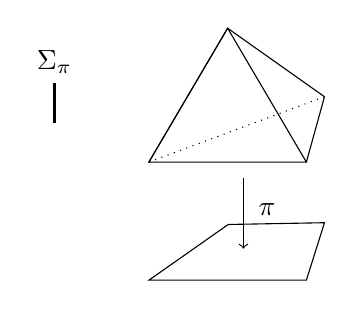
\begin{tikzpicture}		
				\coordinate (A) at (-1.2,1);
				\coordinate (B) at (-1.2,.5);
				\draw[thick] (A) -- (B);
				\node[above] at (A){$\Sigma_\pi$};
				
				% Define the vertices of the 3-simplex
				\coordinate (A) at (0,0);
				\coordinate (B) at (2,0);
				\coordinate (C) at (1, 1.7); 
				\coordinate (D) at (3, 1.6, 2); 
				
				% Draw the edges of the 3-simplex
				\draw (A) -- (B) -- (C) -- cycle;
				\draw (A) -- (C);
				\draw[dotted] (A) -- (D);
				\draw (B) -- (D);
				\draw (C) -- (D);
				
				\draw[<-] (1.2,-1.1) -- (1.2,-.2);
				\node at (1.5, -.6){$\pi$};
				
				% Projection		
				\coordinate (X) at (0,-1.5, 0);
				\coordinate (Y) at (2,-1.5, 0);
				\coordinate (Z) at (1.2, -.6, .5);
				\coordinate (W) at (3, 0, 2);
				
				\draw (X) -- (Y) -- (W) -- (Z) -- cycle;
			\end{tikzpicture}
		\end{center}
	\end{minipage}
	\pause
	\begin{minipage}{.45\textwidth}
		\begin{center}
			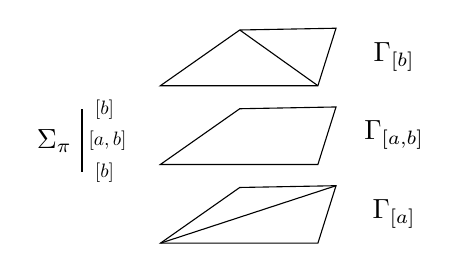
\begin{tikzpicture}		
				\coordinate (A) at (-1,1.2);
				\coordinate (B) at (-1,.4);
				\coordinate (C) at (-1,.8);
				\draw[thick] (A) -- (B);
				
				\node[right,scale=.7] at (A){$\ [b]$};
				\node[right,scale=.7] at (C){$[a,b]$};
				\node[right,scale=.7] at (B){$\ [b]$};
				\node[left] at (C){$\Sigma_\pi$};
				
				% top		
				\coordinate (X) at (0,1.5, 0);
				\coordinate (Y) at (2,1.5, 0);
				\coordinate (Z) at (1.2, 2.4, .5);
				\coordinate (W) at (3, 3, 2);
				
				\draw (X) -- (Y) -- (W) -- (Z) -- cycle;
				\draw (Y) -- (Z);
				
				% middle		
				\coordinate (X) at (0,.5, 0);
				\coordinate (Y) at (2,.5, 0);
				\coordinate (Z) at (1.2, 1.4, .5);
				\coordinate (W) at (3, 2, 2);
				
				\draw (X) -- (Y) -- (W) -- (Z) -- cycle;
				
				% bottom		
				\coordinate (X) at (0,-.5, 0);
				\coordinate (Y) at (2,-.5, 0);
				\coordinate (Z) at (1.2, .4, .5);
				\coordinate (W) at (3, 1, 2);
				
				\draw (X) -- (Y) -- (W) -- (Z) -- cycle;
				\draw (X) -- (W);
				
				\node at (3.2, 2.1, .6){$\Gamma_{[b]}$};
				\node at (3.2, 1.1, .6){$\Gamma_{[a,b]}$};
				\node at (3.2, .1, .6){$\Gamma_{[a]}$};
			\end{tikzpicture}
		\end{center}
	\end{minipage}

	\bigskip\medskip The faces of $\Sigma_\pi$ can be visualized as \colorit{subdivisions} of $Q$.
\end{frame}

\begin{frame}[fragile]{Evaluation}
	\pause
	
	We denote the restriction of polytopal section $\Gamma$ to a face $F$ by $\Gamma(F)$.
	
	\pause\medskip\colorit{Lemma}
	\[
	\begin{tikzcd}[column sep=small, row sep=0]
		\mathrm{ev} \colon &[-10pt] \chains \Sigma_\pi \ot \chains Q \rar & \chains Q \\
		& G \ot F \rar[maps to] & \Gamma_G(F)
	\end{tikzcd}
	\]
	is a chain map.
\end{frame}

\begin{frame}[fragile]{Diagonals polytope}
	\pause
	
	The \colorit{average map}
	\[
	\begin{tikzcd}[column sep=small, row sep=0]
		\alpha \colon &[-20pt] \R^n \times \R^n \rar & \R^n \\
		& v \times w \rar[mapsto]& \frac{v+w}{2}.
	\end{tikzcd}
	\]
	induces a projection $P \times P \to P$ for any $P \subset \R^n$.
	
	\pause\bigskip
	The fiber polytope of this projection is the \colorit{diagonals polytope} $D_P$.
		
	\pause\bigskip
	\colorit{Theorem.} If $D_P$ is framed, then the maps
	\[
	\begin{tikzcd}[column sep=small, row sep=0]
		\triangle_i \colon &[-10pt] \chains P \rar & \chains P \ot \chains P \\
		& F \rar[maps to] & \mathrm{ev}(\so_i(D_P) \ot F)\\
	\end{tikzcd}
	\]
	define a Steenrod diagonal on $P$.
\end{frame}

\begin{frame}{Example}
	\vspace*{-10pt}
	\begin{center}
		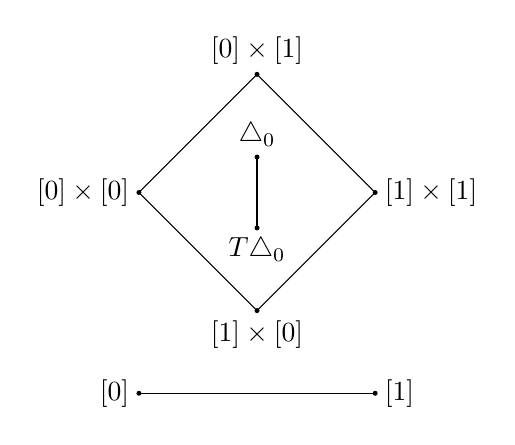
\begin{tikzpicture}[scale=1.5]
			% Shapes
			\coordinate (A) at (1,0);
			\coordinate (B) at (0,1);
			\coordinate (C) at (-1,0);
			\coordinate (D) at (0,-1);
			\draw (A) -- (B) -- (C) -- (D) -- cycle;
			
			\coordinate (X) at (-1,-1.7);
			\coordinate (Y) at (1,-1.7);
			\draw (X) -- (Y);
			
			\coordinate (P) at -- (0,.3);
			\coordinate (Q) at (0,-.3);
			\draw (P) -- (Q);
			
			% Labels
			\node[right,scale=1] at (A) {$[1] \times [1]$};
			\node[above,scale=1] at (B) {$[0] \times [1]$};
			\node[left, scale=1] at (C) {$[0] \times [0]$};
			\node[below,scale=1] at (D) {$[1] \times [0]$};
			
			\node[left,scale=1] at (X) {$[0]$};
			\node[right,scale=1] at (Y) {$[1]$};
			
			\node[above,scale=1] at (P) {$\triangle_0$};
			\node[below,scale=1] at (Q) {$T\triangle_0$};
			
			% Vertices
			\foreach \point in {A, B, C, D, X, Y, P, Q} {
				\fill (\point) circle (.6pt);
			}
		\end{tikzpicture}
	\end{center}

%	\pause\bigskip
%	$\colorit{\triangle_0[01]} = [0] \ot [01] + [01] \ot [1]$
%	\qquad
%	$\colorit{T\triangle_0[01]} = [01] \ot [0] + [1] \ot [01]$
\end{frame}

\begin{frame}[fragile]{Cyclic simplices}
	\pause
	The \colorit{anti-diagonal inclusion} \vspace*{-10pt}
	\[
	\qquad 
	\begin{tikzcd}[column sep=small, row sep=0]
		A \colon &[-20pt] \R^n \rar & \R^n \times \R^n\\
		& v \rar[mapsto]& -v \times v,
	\end{tikzcd}
	\]
	
	\pause
	Let $\colorit{D_n}$ be the diagonals polytope of the cyclic $n$-simplex.
	
	\pause\medskip
	\colorit{Theorem} The frame $\set[\big]{A(e_1),\, A(-e_2),\, A(e_3), \dots}$
	is $D_n$-admissible and \\ the resulting symmetric diagonal is Steenrod's.
	
	\pause
	\begin{center}
		\begin{tikzpicture}	
			% Define the vertices of the triangle
			\coordinate (A) at (0,0);
			\coordinate (B) at (4,0);
			\coordinate (C) at (2,3);
			
			% Calculate the midpoints of the edges
			\coordinate (AB) at ($(A)!0.5!(B)$);
			\coordinate (BC) at ($(B)!0.5!(C)$);
			\coordinate (AC) at ($(C)!0.5!(A)$);
			
			% subdivisions
			\draw (A) -- (B) -- (C) -- cycle;
			\draw (AB) -- (AC);
			\draw (AC) -- (BC);
			
			\coordinate (ABC) at ($ (A)!.333!(AB)!.333!(AC) $);
			\coordinate (CBA) at ($ (AC)!.333!(BC)!.333!(C) $);
			\coordinate (CAB) at ($ (AB)!0.25!(B)!0.25!(BC)!0.25!(AC) $);
			
			% Optionally, label the vertices and midpoints
			\node[below left] at (A) {$0|0$};
			\node[below right] at (B) {$1|1$};
			\node[above] at (C) {$2|2$};
			\node[below] at (AB) {$0|1$};
			\node[left] at (AC) {$0|2$};
			\node[right] at (BC) {$1|2$};
			\node at (ABC) {\quad $0|012$};
			\node at (CBA) {\quad $012|2$};
			\node at (CAB) {\quad $01|12$};
		\end{tikzpicture}
	\end{center}
\end{frame}




%\begin{frame}{Oriented posets}
%	\pause
%	Let $(\Gamma, \leq)$ be a poset and $z \in \Gamma$.
%	The \colorit{cover set} of $z$:
%	\[
%	\cov(z) = \set{x < z \mid \nexists y,\ x < y < z}.
%	\]
%
%	\pause
%	An \colorit{orientation} is a partition $\so(z) \sqcup \ta(z) = \cov(z)$ for each $z \in P$.
%
%	\pause\bigskip
%	\colorit{Construction} An orientation $\omega$ of $P$ induces an orientation on $\faces(P)$.
%
%	\pause
%	\[
%	\text{Facet } E \leq F \text{ in } \ta(F) \qquad iff \qquad \omega_F \sim (\normal_E^F \wedge \, \omega_E).
%	\]
%
%	\pause\bigskip
%	\colorit{Ambiguity} This orientation on $\faces(P)$ determines $\omega$ up to
%	\[
%	\forall F,\ \omega_F \mapsto - \omega_F.
%	\]
%\end{frame}
%
%\begin{frame}{Refinement systems}
%	\pause
%	A \colorit{poset refinement system} is a collection $\set{\leq_i}$ of poset relations on $X$~s.t.
%	\[
%	\id \colon (X, \leq_i) \to (X, \leq_j)
%	\]
%	is order-preserving for $i \leq j$.
%
%	\pause\medskip
%	\colorit{Construction} If $P$ is framed then $\faces(P)$ has a poset refinement system.
%
%	\pause
%	\[
%	F \leq_k G \qquad iff \qquad \pi_k(F) \subseteq \pi_k(G)
%	\]
%
%	\pause\smallskip
%	Each poset $(\faces(P), \leq_k)$ has a canonical orientation induced by the frame.
%	\[
%	\pi_k(F),
%	\]
%
%	\pause\medskip
%	For $F \in \faces(P)$ say $\dim f = m$, then $k$-source and $k$-target of $F \in \faces(P)$
%	\[
%	\so_k(F) = {}
%	\]
%
%\end{frame}
